On étudie le problème d'optimisation qui consiste à optimiser le diagramme $D(\theta)$ d'une antenne. Il s'agit de trouver les coefficients d'amplification $x_i$ des $N$ anneaux de l'antenne qui satisfassent aux conditions de diagramme unitaire (dans l'intervalle $\mathcal{P}=[\theta_P, 90\degree]$) ou nul (dans l'intervalle $\mathcal{S}=[0 \degree,\theta_S]$).

\section{Formulation linéaire}
\subsection{Modèle}
On peut formuler le programme d'optimisation comme suit :
\begin{align}
\min_{x_i,\epsilon} \epsilon & \\
&|D(\theta)-1|  \leq \epsilon &\forall \theta\in \mathcal{P}\\
&|D(\theta)| \leq \epsilon & \forall \theta\in \mathcal{S}\label{conS}\\
& \epsilon \geq 0\\
\text{avec } D(\theta) = \sum_{i=1}^N x_i d_i(\theta) & \text{ et } d_i(\theta) = \int_0^{2 \pi} cos(2 \pi r_i cos(\theta)cos(\phi)) d\phi \label{eq:di}
\end{align}
Le problème posé présente un désavantage majeur; il est soumis à une infinité de contraintes (\ref{conS}).\\
Pour pallier à ce problème, nous échantillonnons le problème par rapport à $\theta$. Les contraintes du problèmes ne s'appliquant que dans $P = [\theta_P\: 90\degres  ]$ et $S = [0\degres \:\theta_S]$, nous échantillonnons seulement dans ces deux ensembles. Nous avons ainsi un nombre fini de contraintes. Afin de n'obtenir que des contraintes linéaires, nous transformons chaque contrainte faisant intervenir une valeur absolue en deux contraintes linéaires. Le problème devient alors : 
\begin{align}
\min_{x_i,\epsilon} \epsilon & & \nonumber\\
& D(\theta)-1\leq \epsilon & \forall \theta\in \mathcal{P}_e \\
& -D(\theta)+1\leq \epsilon & \forall \theta\in \mathcal{P}_e\\
& D(\theta)\leq \epsilon & \forall \theta\in \mathcal{S}_e\\
& -D(\theta)\leq \epsilon &\forall \theta\in \mathcal{S}_e\\
\text{avec } D(\theta) = \sum_{i=1}^N x_i d_i(\theta) & \text{ et } d_i(\theta) = \int_0^{2 \pi} cos(2 \pi r_i cos(\theta)cos(\phi)) d\phi 
\end{align}
$\mathcal{P}_e = \left\lbrace p_0,p_1,...,p_{Np}\right\rbrace$ et $\mathcal{S}_e= \left\lbrace s_0,s_1,...,s_{Ns}\right\rbrace$ sont les ensembles des échantillons dans $\mathcal{P}$ et $\mathcal{S}$. Deux points consécutifs sont séparés par une distance maximale de $h$.\\
Cette formulation est bien évidemment une formulation approchée de notre problème initial puisque des points entre les échantillons pourront ne pas satisfaire les contraintes de diagramme unitaire ou nul. Cependant le non-respect de ces contraintes peut être quantifié. En effet, d'après les définitions des $d_i(\theta)$, la valeur absolue de la dérivée de ceux-ci ne peut pas dépasser $\pi$. Ce qui signifie que le dépassement de l'erreur de diagramme est au maximum $\sum |x_i\pi h|$. Il nous suffit alors de choisir un $h$ adapté au niveau de précision que nous voulons atteindre. 
\\
Notons que lors de l'implémentation de notre modèle, nous faisons une deuxième approximation en calculant les diagrammes $d_i(\theta)$. Comme l'intégrale de l'équation \eqref{eq:di} n'est pas calculable analytiquement (il s'agit d'une fonction de Bessel), nous la calculons numériquement au moyen d'une somme de Rieman dans notre code Ampl.
\textbf{Todo : Expliquer notre choix de h, trouver une meilleure borne?, résoudre en ampl}		\\

\subsection{Analyse des résultats}
La figure \ref{fig:D-ModLin} donne une illustration des diagrammes optimaux obtenus pour certains paramètres. On constate que lorsque $\theta_P$ et $\theta_S$ deviennent proches, le $\epsilon$ croit. On remarque également que tous les points $\in \mathcal{S}$ ou $\in \mathcal{P}$ sont bien compris entre les bornes fixées par $\epsilon$; et ce malgré que nous ayons discrétisé le problème et que nous n'ayons donc pas imposer cette contrainte pour tous les points. Cela confirme l'idée que l'approximation faite est acceptable. Définissons l'erreur du diagramme $D(\theta)$ comme suit : 
\begin{equation} \label{eq:erreurDiagramme}
err = \int _{\mathcal{S}} |D(\theta)| d\theta + \int_{\mathcal{P}} |D(\theta) - 1| d\theta.
\end{equation}
On obtient 0.0209 (en bleu) et 0.1151 (vert) comme erreur pour les diagrammes de la figure \ref{fig:D-ModLin}. Pour les $x$ perturbés, on obtient comme erreur moyenne 6.5605 pour les diagrammes de la figure \ref{fig:D-ModLin-RobustTau01} et 64.6476 pour les diagrammes de la figure \ref{fig:D-ModLin-RobustTau01}.
\begin{figure}[h!]
  \centering
  \begin{subfigure}[b]{0.32\textwidth}
  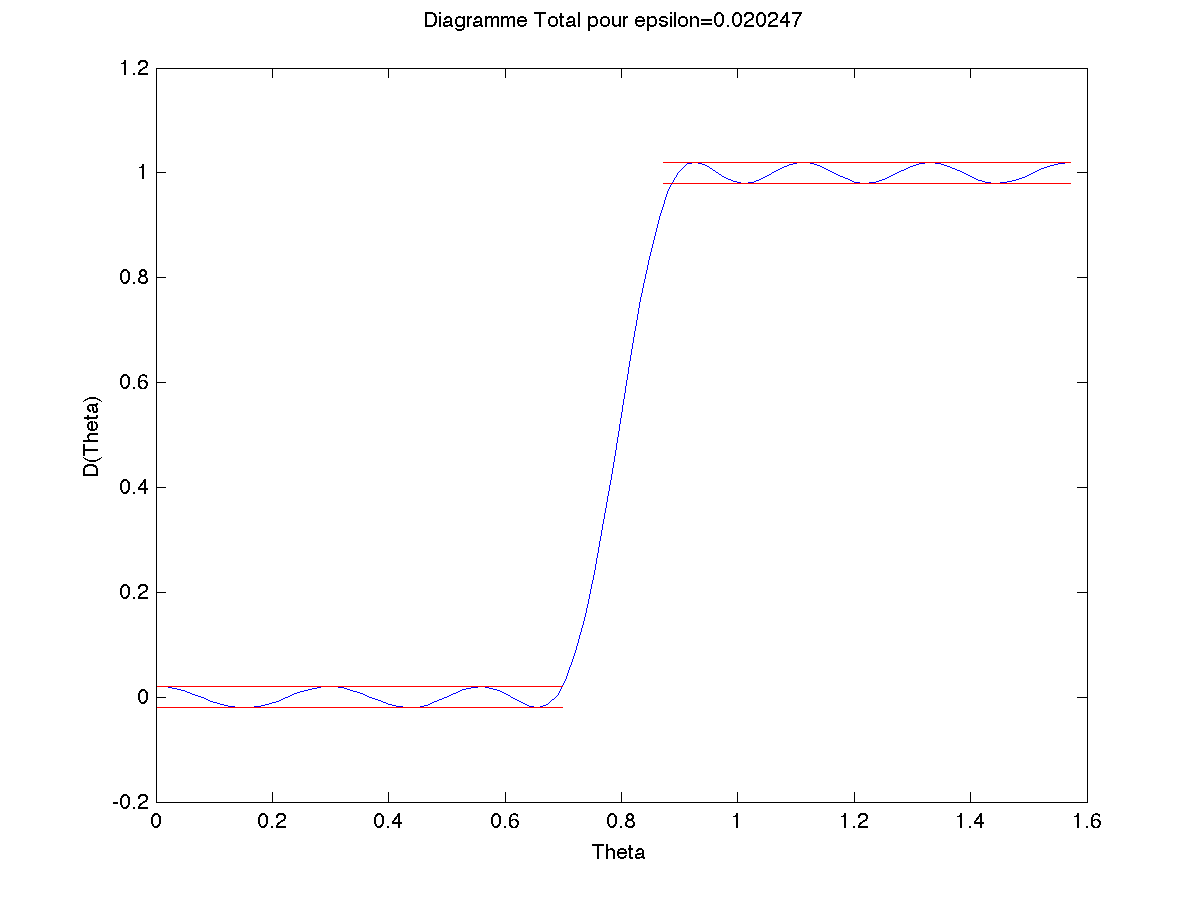
\includegraphics[width=\textwidth]{D-ModLin.png}
  \caption{Diagramme optimal $D(\theta)$ de l'antenne composé de 40 anneaux, pour $r_i=i/10$. En bleu pour $\theta_P=50 \degree$ et $\theta_S=40 \degree$; en vert pour $\theta_P=47 \degree$ et $\theta_S=43 \degree$. En rouge, les bornes du $\epsilon$ optimal trouvé (en bleu $2.4 \%$, en vert $11.9 \%$).}
  \label{fig:D-ModLin}
  \end{subfigure}%
  ~ 
  \begin{subfigure}[b]{0.32\textwidth}
  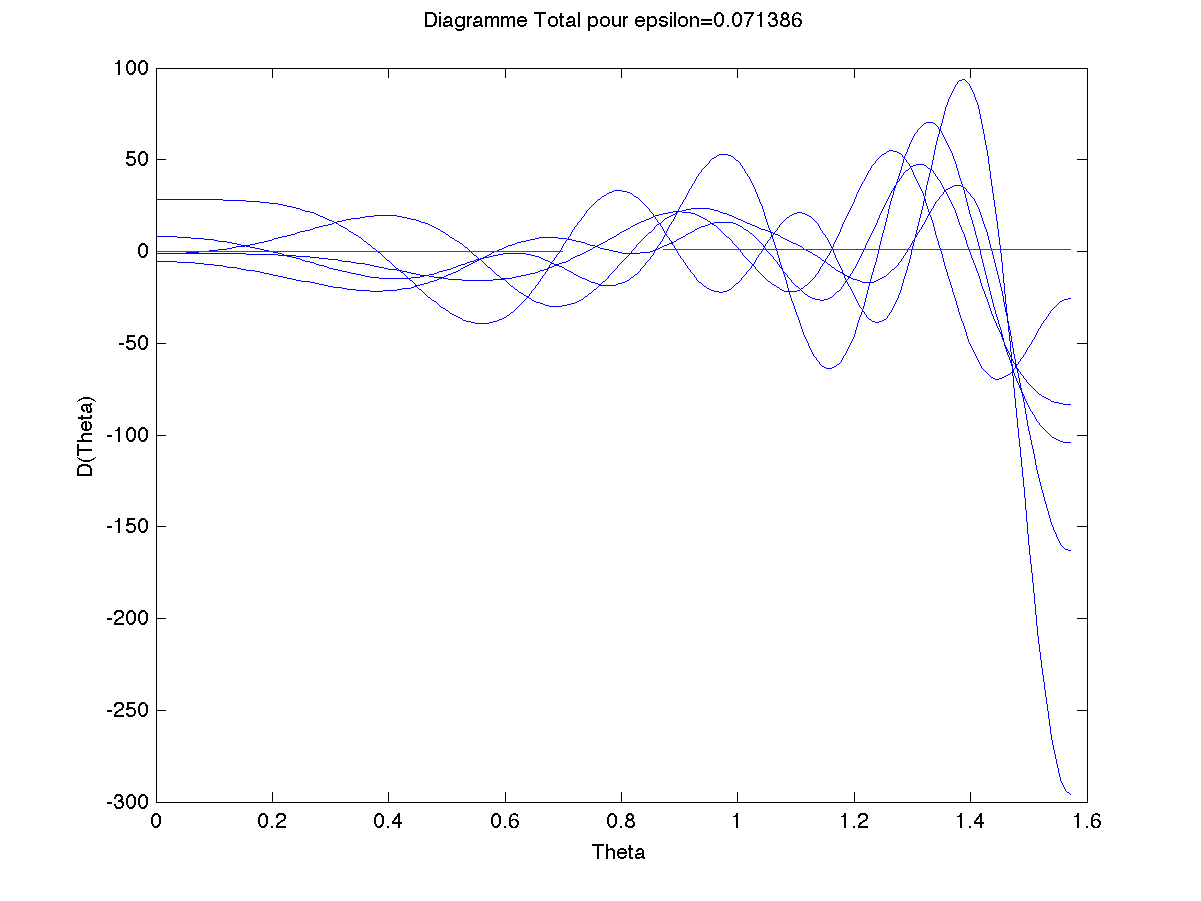
\includegraphics[width=\textwidth]{D-ModLin-2RobustTau01.png}
  \caption{Diagramme optimal $D(\theta)$ de l'antenne composé de 40 anneaux, pour $r_i=i/10$, $\theta_P=50 \degree$ et $\theta_S=40 \degree$ avec un vecteur $x$ perturbé ($\tau = 0.01$).}
  \label{fig:D-ModLin-RobustTau01}
  \end{subfigure}
   ~ 
  \begin{subfigure}[b]{0.32\textwidth}
  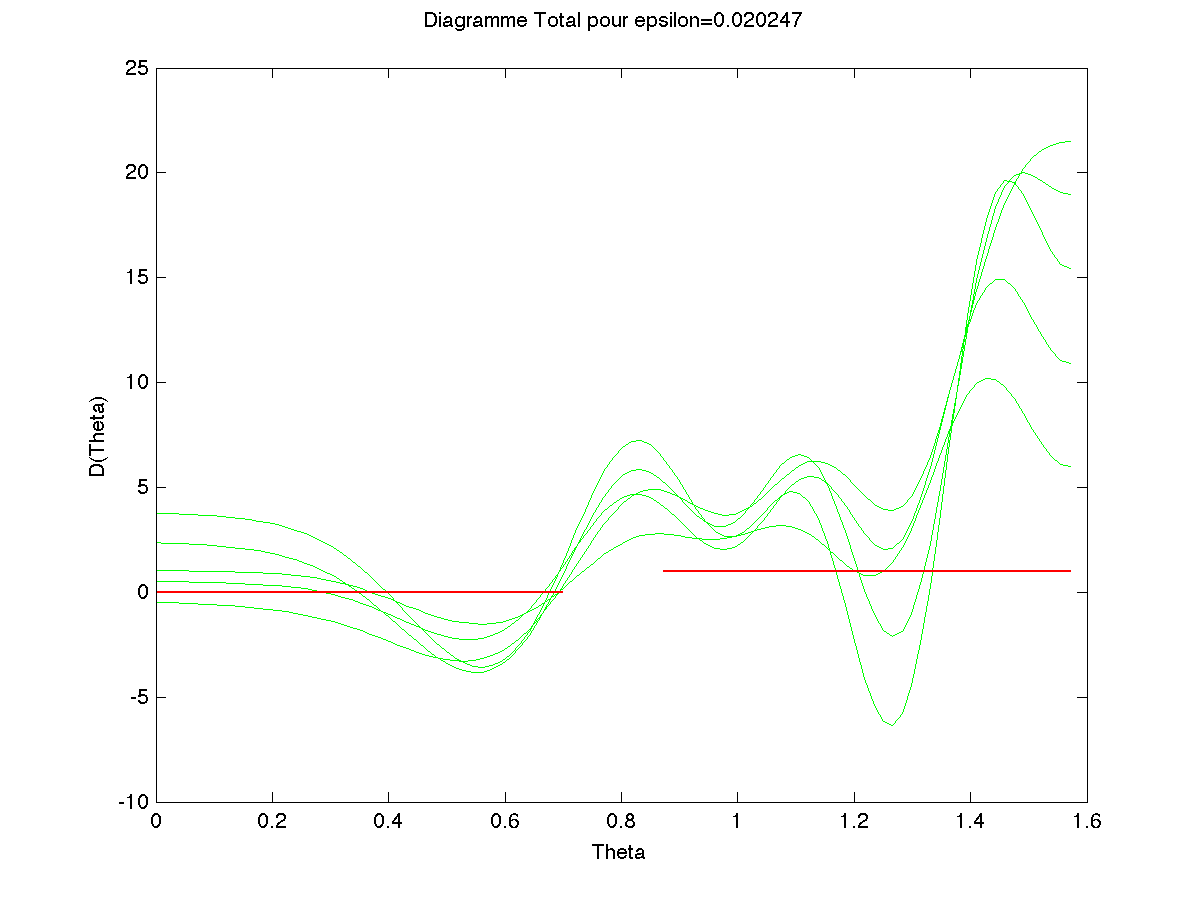
\includegraphics[width=\textwidth]{D-ModLin-2RobustTau001.png}
  \caption{Diagramme optimal $D(\theta)$ de l'antenne composé de 40 anneaux, pour $r_i=i/10$, $\theta_P=50 \degree$ et $\theta_S=40 \degree$ avec un vecteur $x$ perturbé ($\tau=0.001$).}
  \label{fig:D-ModLin-RobustTau001}
  \end{subfigure}
  \caption{}
  \end{figure}


\subsection{Analyse de la robustesse}
En pratique, l'implémentation des $x_i$ n'est pas réalise parfaitement. On a plutôt $\hat{x}_i = x_i(1+\xi_i)$ où les erreurs $\xi_i$ se situent dans un intervalle $[-\tau,\tau]$.\\
Reprenons le modèle linéaire précédent et appliquons-lui des erreurs $xi_i$ de l'ordre de $\tau=0.001$ et $\tau=0.01$. On obtient les graphes aux figures \ref{fig:D-ModLin-RobustTau01} et \ref{fig:D-ModLin-RobustTau001}. On a donc une solution très sensible aux perturbations. Une valeur des erreurs sont données aux tableau récapitulatif \ref{table:Recap}. Ce tableau nous donne aussi une indication sur l'ordre de grandeur des $x_i$. Ils sont très élevé dans notre cas. Intuitivement, un grand $x_i$ positif vient compenser un grand $x_i$ négatif... dés qu'on perturbe ces valeurs des $x$, on a directement de grandes erreurs. On peut supposer qu'on modèle plus robuste consisterait à réduire ces valeurs ces $x_i$.









